\subsection{Abas}


\subsubsection{Abas simples}

Organização de texto horizontalmente com foco num tópico por vez.

\begin{figure}[!ht]
    \centering
    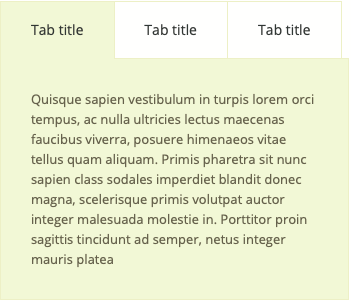
\includegraphics[scale=.5]{abas-simples}
    \caption{Abas simples}\label{RS0001:fig:abas-simples}
\end{figure}

\begin{code}
    \inputminted[label=abas-slide.html]{html}{../RS0001/anexos/abas-simples.html}
    \caption{Exemplo de abas simples}\label{RS0001:code:exemplo-abas-simples}
\end{code}


\subsubsection{Abas (slide)}

Igual à aba simples, porém acrescenta o efeito de deslizamento lateral na mudança de aba. Observe que houve uma quebra de linha nas abas pois os títulos ocuparam um espaço maior que o reservado.

\begin{figure}[!ht]
    \centering
    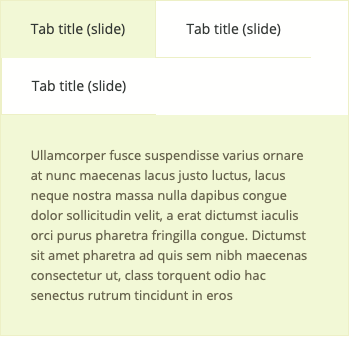
\includegraphics[scale=.5]{abas-slide}
    \caption{Abas (slide)}\label{RS0001:fig:abas-slide}
\end{figure}

\begin{code}
    \inputminted[label=abas-slide.html]{html}{../RS0001/anexos/abas-slide.html}
    \caption{Exemplo de abas (slide)}\label{RS0001:code:exemplo-abas-slide}
\end{code}


\subsubsection{Abas (longas)}

Abas ocupando a largura total da publicação.

\begin{figure}[!ht]
    \centering
    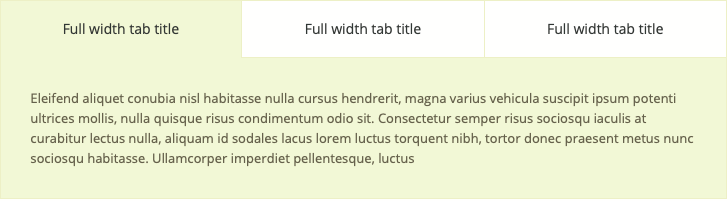
\includegraphics[scale=.5]{abas-longa}
    \caption{Abas (longas)}\label{RS0001:fig:abas-longa}
\end{figure}

\begin{code}
    \inputminted[label=abas-longa.html]{html}{../RS0001/anexos/abas-longa.html}
    \caption{Exemplo de abas (longa)}\label{RS0001:code:exemplo-abas-longa}
\end{code}


\subsubsection{Abas verticais simples}

Organização do texto verticalmente com foco num tópico por vez. Observe que houve uma quebra de linha nas abas pois os títulos ocuparam um espaço maior que o reservado.

\begin{figure}[!ht]
    \centering
    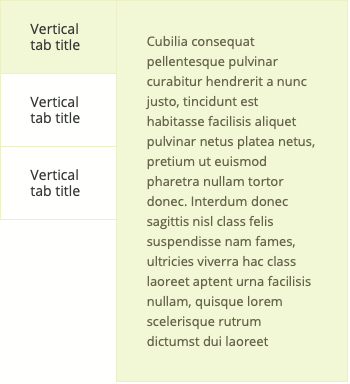
\includegraphics[scale=.5]{abas-vertical-simples}
    \caption{Abas verticais simples}\label{RS0001:fig:abas-vertical-simples}
\end{figure}

\begin{code}
    \inputminted[label=abas-vertical-simples.html]{html}{../RS0001/anexos/abas-vertical-simples.html}
    \caption{Exemplo de abas verticais simples}\label{RS0001:code:exemplo-abas-vertical-simples}
\end{code}


\subsubsection{Abas verticais (slide)}

Igual à aba vertical simples, porém acrescenta o efeito de deslizamento longitudinal na mudança de aba. Observe que houve uma quebra de linha nas abas pois os títulos ocuparam um espaço maior que o reservado.

\begin{figure}[!ht]
    \centering
    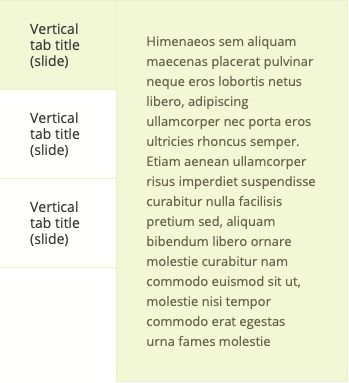
\includegraphics[scale=.5]{abas-vertical-slide}
    \caption{Abas verticais simples (slide)}\label{RS0001:fig:abas-vertical-slide}
\end{figure}

\begin{code}
    \inputminted[label=abas-vertical-slide.html]{html}{../RS0001/anexos/abas-vertical-slide.html}
    \caption{Exemplo de abas verticais (slide)}\label{RS0001:code:exemplo-abas-vertical-slide}
\end{code}


\subsubsection{Abas coloridas simples}

\begin{figure}[!ht]
    \centering
    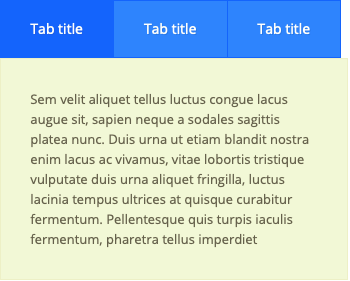
\includegraphics[scale=.5]{abas-coloridas-simples}
    \caption{Abas coloridas simples}\label{RS0001:fig:abas-coloridas-simples}
\end{figure}

\begin{code}
    \inputminted[label=abas-abas-coloridas-simples.html]{html}{../RS0001/anexos/abas-coloridas-simples.html}
    \caption{Exemplo de abas coloridas simples}\label{RS0001:code:exemplo-abas-coloridas-simples}
\end{code}


\subsubsection{Abas coloridas (slide)}

\begin{figure}[!ht]
    \centering
    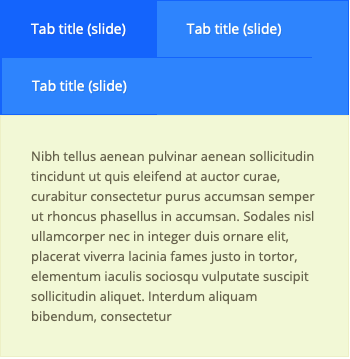
\includegraphics[scale=.5]{abas-coloridas-slide}
    \caption{Abas coloridas (slide)}\label{RS0001:fig:abas-coloridas-slide}
\end{figure}

\begin{code}
    \inputminted[label=abas-abas-coloridas-slide.html]{html}{../RS0001/anexos/abas-coloridas-slide.html}
    \caption{Exemplo de abas coloridas (slide)}\label{RS0001:code:exemplo-abas-coloridas-slide}
\end{code}


\subsubsection{Abas coloridas (longas)}

\begin{figure}[!ht]
    \centering
    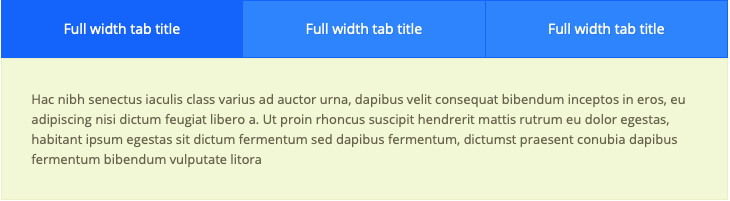
\includegraphics[scale=.5]{abas-coloridas-longa}
    \caption{Abas coloridas (longas)}\label{RS0001:fig:abas-coloridas-longa}
\end{figure}

\begin{code}
    \inputminted[label=abas-abas-coloridas-longa.html]{html}{../RS0001/anexos/abas-coloridas-longa.html}
    \caption{Exemplo de abas coloridas (longas)}\label{RS0001:code:exemplo-abas-coloridas-longa}
\end{code}


\subsubsection{Abas coloridas verticais simples}

\begin{figure}[!ht]
    \centering
    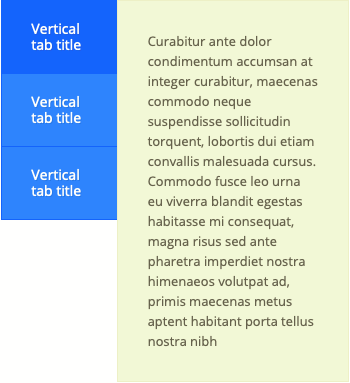
\includegraphics[scale=.5]{abas-coloridas-vertical-simples}
    \caption{Abas coloridas verticais simples}\label{RS0001:fig:abas-coloridas-vertical-simples}
\end{figure}

\begin{code}
    \inputminted[label=abas-abas-coloridas-vertical-simples.html]{html}{../RS0001/anexos/abas-coloridas-vertical-simples.html}
    \caption{Exemplo de abas coloridas verticais simples}\label{RS0001:code:exemplo-abas-coloridas-vertical-simples}
\end{code}


\subsubsection{Abas coloridas verticais (slide)}

\begin{figure}[!ht]
    \centering
    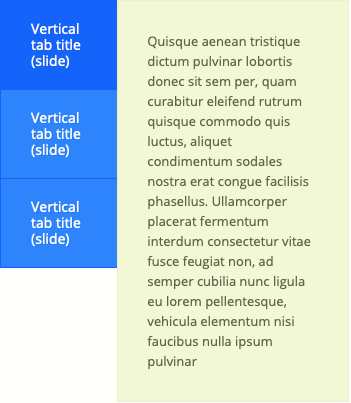
\includegraphics[scale=.5]{abas-coloridas-vertical-slide}
    \caption{Abas coloridas verticais (slide)}\label{RS0001:fig:abas-coloridas-vertical-slide}
\end{figure}

\begin{code}
    \inputminted[label=abas-abas-coloridas-vertical-slide.html]{html}{../RS0001/anexos/abas-coloridas-vertical-slide.html}
    \caption{Exemplo de abas coloridas verticais (slide)}\label{RS0001:code:exemplo-abas-coloridas-vertical-slide}
\end{code}